\documentclass{article}
\usepackage[final]{nips_2017}
\usepackage{polski}
\usepackage[utf8]{inputenc}    % allow utf-8 input
\usepackage[T1]{fontenc}       % use 8-bit T1 fonts
\usepackage{hyperref}          % hyperlinks
\usepackage{url}               % simple URL typesetting
\usepackage{booktabs}          % professional-quality tables
\usepackage{amsfonts}          % blackboard math symbols
\usepackage{nicefrac}          % compact symbols for 1/2, etc.
\usepackage{microtype}         % microtypography
\usepackage[section]{placeins} % figures kept in sections
\usepackage{graphicx}          % images
\graphicspath{ {./img/} }
\usepackage{multirow}

\renewcommand{\figurename}{Wykres}

\title{  Sieć wielowarstwowa\\Sieci Neuronowe 2020 }

\author{
  Jakub Ciszek \\
  238035\\
}

% TODO images

\begin{document}

\maketitle

\newpage
\tableofcontents
\newpage

Cały kod wykorzystany w zadaniu znajduje się pod adresem: \url{https://github.com/Greenpp/sieci-neuronowe-pwr-2020}

\section{Opis badań}
\subsection{Plan eksperymentów}

Wszystkie eksperymenty zostały przeprowadzone 10 razy. Losowość przy inicjalizacji wag oraz generacji danych nie została narzucona żadnym ziarnem. Podczas badań przyjęto górną granicę 1 epoki, po przekroczeniu której, uczenie zostawało przerywane. Ze względu na charakter zadania (klasyfikacja) na ostatniej warstwie użyto funkcji Softmax, a za funkcję straty przyjęto Entropię krzyżową.
Z powodów wydajnościowych testowanie modelu przeprowadzano co każde 1024 przykłady.\\
Zgodnie z instrukcją zostały przeprowadzone następujące badania:
\begin{itemize}
	\item Wpływ wielkości warstwy ukrytej na przebieg procesu uczenia
	\item Wpływ wielkości paczki na przebieg procesu uczenia
	\item Wpływ zakresu inicjalizacji wag na przebieg procesu uczenia
	\item Wpływ wartości współczynnika alpha na przebieg procesu uczenia
	\item Wpływ użytej funkcji aktywacyjnej na przebieg procesu uczenia
	      	      	      	      	      	      	      	      	      	      	      	      	      	
\end{itemize}

\subsection{Charakterystyka zbiorów danych}

Danymi użytymi w zadaniu jest zbiór ręcznie pisanych cyfr \(0-9\) - MNIST. Na zbiór składa się 70,000 obrazów wielkości 28x28 pikseli, co po przekształceniu odpowiadało 784 elementowemu wektorowi wejściowemu. Użyta w zadaniu wersja została podzielona na 3 zbiory:
\begin{itemize}
	\item Uczący - 50,000 przykładów.
	\item Walidujący - 10,000 przykładów.
	\item Testowy - 10,000 przykładów.
\end{itemize}
W trakcie eksperymentów wykorzystano jedynie zbiory uczący i testowy.

\newpage
\section{Eksperymenty}

\subsection{Wpływ wielkości warstwy ukrytej na przebieg procesu uczenia}
\subsubsection*{Założenia}
\begin{table}[!h]
	\caption{Stałe dla eksperymentu 1}
	\label{tabela-const-1}
	\centering
	\begin{tabular}{lr}
		\toprule
		Parametr               & Wartość         \\
		\midrule
		Wielkość paczki      & 32                \\
		Zakres wag             & \($-0.5 -- 0.5$\) \\
		Współczynnik uczenia & 0.01              \\
		Funkcja aktywacji      & ReLU              \\
		\bottomrule
	\end{tabular}
\end{table}

Zmienną w tym eksperymencie była wielkość warstwy ukrytej. Ilość neuronów przyjmowała wartości ze zbioru \(\{$16, 128, 512, 2048$\}\)
\subsubsection*{Przebieg}

Podczas eksperymentu model został zainicjalizowany 10 razy dla każdej z badanych wartości oraz wyuczony, uzyskane wyniki zostały zapisane w postaci pliku .plk do dalszej analizy.

\subsubsection*{Wyniki}
\begin{figure}[!h]
	\centering
	\caption{Przebieg procesu uczenia w zależności od wielkości warstwy ukrytej}
	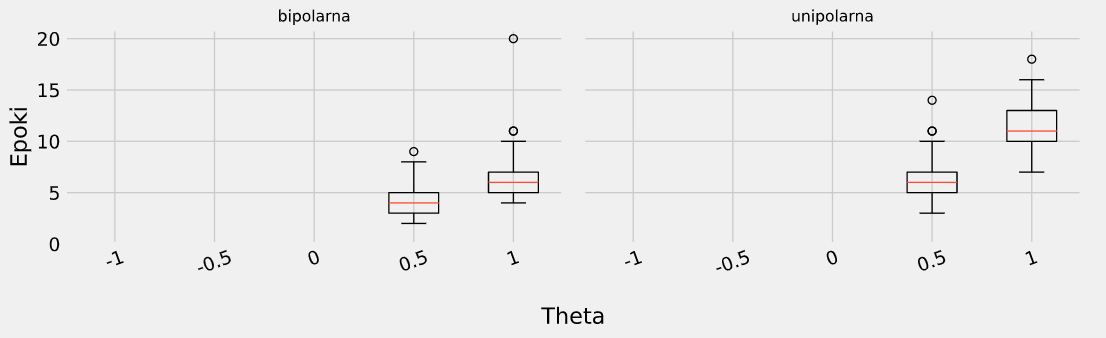
\includegraphics[width=\textwidth]{per_theta.png}
	\label{fig:res11}
\end{figure}

\begin{table}[!h]
	\caption{Średnia maksymalna dokładność w zależności od wielkości warstwy ukrytej}
	\label{tabela-res-11}
	\centering
	\begin{tabular}{rrr}
		\toprule
		Neurony & Dokładność \\
		\midrule
		16      & -             \\
		128     & -             \\
		512     & -             \\
		2048    & -             \\
		\bottomrule
	\end{tabular}
\end{table}

\subsubsection*{Wnioski}

Z otrzymanych wyników, widocznych na wykresie~\ref{fig:res11} oraz tabeli~\ref{tabela-res-11}, wynika że

\newpage
\subsection{Wpływ wielkości paczki na przebieg procesu uczenia}
\subsubsection*{Założenia}
\begin{table}[!h]
	\caption{Stałe dla eksperymentu 2}
	\label{tabela-const-2}
	\centering
	\begin{tabular}{lr}
		\toprule
		Parametr                   & Wartość         \\
		\midrule
		Wielkość warstwy ukrytej & 128               \\
		Zakres wag                 & \($-0.5 -- 0.5$\) \\
		Współczynnik uczenia     & 0.01              \\
		Funkcja aktywacji          & ReLU              \\
		\bottomrule
	\end{tabular}
\end{table}

Zmienną w tym eksperymencie była wielkość paczki. Ilość przykładów przyjmowała wartości ze zbioru \(\{$1, 8, 32, 128, 1024$\}\)
\subsubsection*{Przebieg}

Podczas eksperymentu model został zainicjalizowany 10 razy dla każdej z badanych wartości oraz wyuczony, uzyskane wyniki zostały zapisane w postaci pliku .plk do dalszej analizy.

\subsubsection*{Wyniki}
\begin{figure}[!h]
	\centering
	\caption{Przebieg procesu uczenia w zależności od wielkości paczki}
	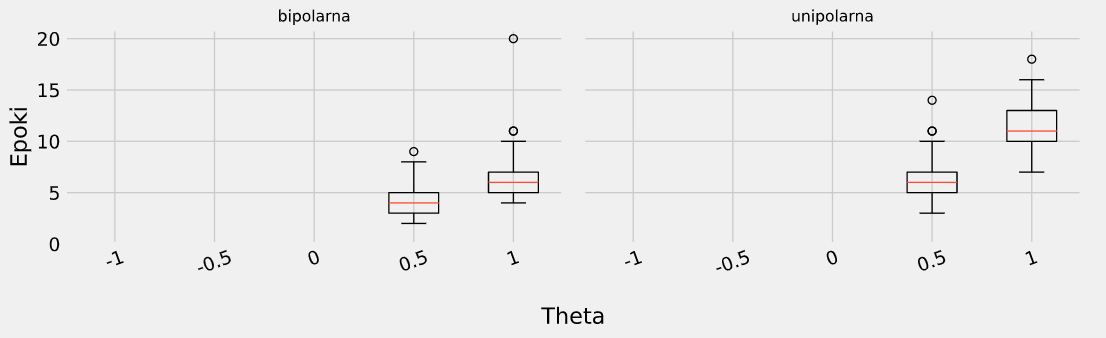
\includegraphics[width=\textwidth]{per_theta.png}
	\label{fig:res21}
\end{figure}

\begin{table}[!h]
	\caption{Średnia maksymalna dokładność w zależności od wielkości paczki}
	\label{tabela-res-21}
	\centering
	\begin{tabular}{rrr}
		\toprule
		Przykłady & Dokładność \\
		\midrule
		1          & -             \\
		8          & -             \\
		32         & -             \\
		128        & -             \\
		1024       & -             \\
		\bottomrule
	\end{tabular}
\end{table}

\subsubsection*{Wnioski}

Z otrzymanych wyników, widocznych na wykresie~\ref{fig:res21} oraz tabeli~\ref{tabela-res-21}, wynika że

\newpage
\subsection{Wpływ zakresu inicjalizacji wag na przebieg procesu uczenia}
\subsubsection*{Założenia}
\begin{table}[!h]
	\caption{Stałe dla eksperymentu 3}
	\label{tabela-const-3}
	\centering
	\begin{tabular}{lr}
		\toprule
		Parametr                   & Wartość \\
		\midrule
		Wielkość warstwy ukrytej & 128       \\
		Wielkość paczki          & 32        \\
		Współczynnik uczenia     & 0.01      \\
		Funkcja aktywacji          & ReLU      \\
		\bottomrule
	\end{tabular}
\end{table}

Zmienną w tym eksperymencie był zakres inicjalizacji wag. Przedział inicjalizacji przyjmował wartości ze zbioru \(\{$0.0, -0.1 -- 0.1, -0.5 -- 0.5, -2.0 -- 2.0$\}\)
\subsubsection*{Przebieg}

Podczas eksperymentu model został zainicjalizowany 10 razy dla każdej z badanych wartości oraz wyuczony, uzyskane wyniki zostały zapisane w postaci pliku .plk do dalszej analizy.

\subsubsection*{Wyniki}
\begin{figure}[!h]
	\centering
	\caption{Przebieg procesu uczenia w zależności od zakresu inicjalizacji wag}
	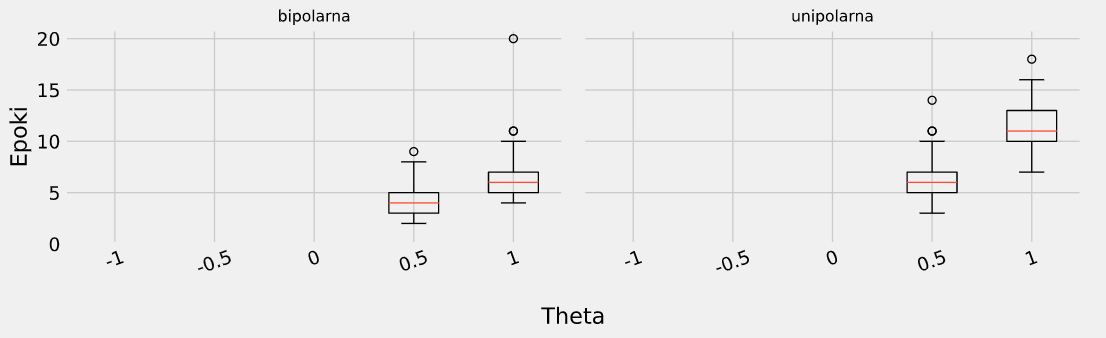
\includegraphics[width=\textwidth]{per_theta.png}
	\label{fig:res31}
\end{figure}

\begin{table}[!h]
	\caption{Średnia maksymalna dokładność w zależności od zakresu inicjalizacji wag}
	\label{tabela-res-31}
	\centering
	\begin{tabular}{rrr}
		\toprule
		Zakres            & Dokładność \\
		\midrule
		0.0               & -             \\
		\($-0.1 -- 0.1$\) & -             \\
		\($-0.5 -- 0.5$\) & -             \\
		\($-2.0 -- 2.0$\) & -             \\
		\bottomrule
	\end{tabular}
\end{table}

\subsubsection*{Wnioski}

Z otrzymanych wyników, widocznych na wykresie~\ref{fig:res31} oraz tabeli~\ref{tabela-res-31}, wynika że

\newpage
\subsection{Wpływ wartości współczynnika alpha na przebieg procesu uczenia}
\subsubsection*{Założenia}
\begin{table}[!h]
	\caption{Stałe dla eksperymentu 4}
	\label{tabela-const-4}
	\centering
	\begin{tabular}{lr}
		\toprule
		Parametr                   & Wartość         \\
		\midrule
		Wielkość warstwy ukrytej & 128               \\
		Wielkość paczki          & 32                \\
		Zakres wag                 & \($-0.5 -- 0.5$\) \\
		Funkcja aktywacji          & ReLU              \\
		\bottomrule
	\end{tabular}
\end{table}

Zmienną w tym eksperymencie był współczynnik uczenia. Przyjmował wartości ze zbioru \(\{$0.0001, 0.001, 0.01, 0.1, 1.0,$\}\)
\subsubsection*{Przebieg}

Podczas eksperymentu model został zainicjalizowany 10 razy dla każdej z badanych wartości oraz wyuczony, uzyskane wyniki zostały zapisane w postaci pliku .plk do dalszej analizy.

\subsubsection*{Wyniki}
\begin{figure}[!h]
	\centering
	\caption{Przebieg procesu uczenia w zależności od współczynnika uczenia}
	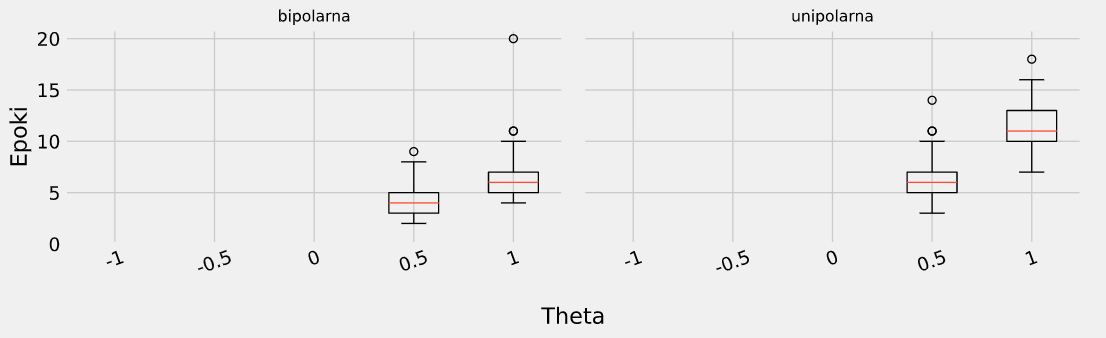
\includegraphics[width=\textwidth]{per_theta.png}
	\label{fig:res41}
\end{figure}

\begin{table}[!h]
	\caption{Średnia maksymalna dokładność w zależności od współczynnika uczenia}
	\label{tabela-res-41}
	\centering
	\begin{tabular}{rrr}
		\toprule
		Alpha  & Dokładność \\
		\midrule
		0.0001 & -             \\
		0.0010 & -             \\
		0.0100 & -             \\
		0.1000 & -             \\
		1.0000 & -             \\
		\bottomrule
	\end{tabular}
\end{table}

\subsubsection*{Wnioski}

Z otrzymanych wyników, widocznych na wykresie~\ref{fig:res41} oraz tabeli~\ref{tabela-res-41}, wynika że

\newpage
\subsection{Wpływ użytej funkcji aktywacyjnej na przebieg procesu uczenia}
\subsubsection*{Założenia}
\begin{table}[!h]
	\caption{Stałe dla eksperymentu 5}
	\label{tabela-const-5}
	\centering
	\begin{tabular}{lr}
		\toprule
		Parametr                   & Wartość         \\
		\midrule
		Wielkość warstwy ukrytej & 128               \\
		Wielkość paczki          & 32                \\
		Zakres wag                 & \($-0.5 -- 0.5$\) \\
		Współczynnik uczenia     & 0.01              \\
		\bottomrule
	\end{tabular}
\end{table}

Zmienną w tym eksperymencie była funkcja aktywacji. Przetestowane zostały funkcje Sigmoidalna oraz ReLU.
\subsubsection*{Przebieg}

Podczas eksperymentu model został zainicjalizowany 10 razy dla każdej z badanych wartości oraz wyuczony, uzyskane wyniki zostały zapisane w postaci pliku .plk do dalszej analizy.

\subsubsection*{Wyniki}
\begin{figure}[!h]
	\centering
	\caption{Przebieg procesu uczenia w zależności od funkcji aktywacji}
	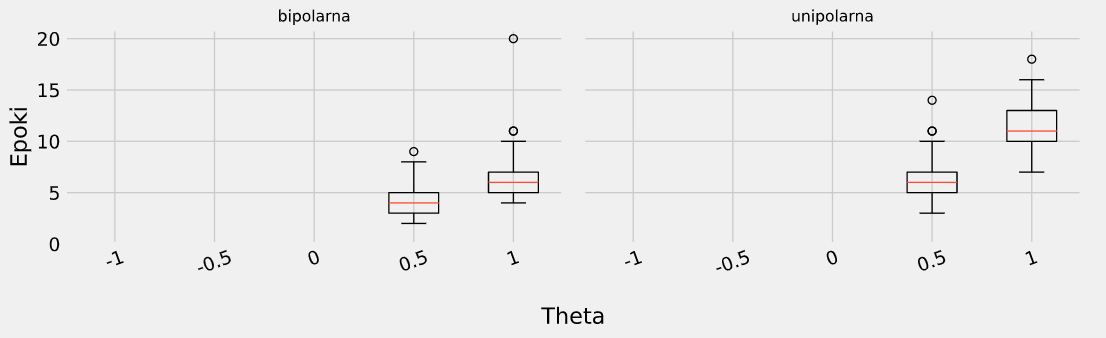
\includegraphics[width=\textwidth]{per_theta.png}
	\label{fig:res51}
\end{figure}

\begin{table}[!h]
	\caption{Średnia maksymalna dokładność w zależności od funkcji aktywacji}
	\label{tabela-res-51}
	\centering
	\begin{tabular}{rrr}
		\toprule
		Funkcja & Dokładność \\
		\midrule
		Sigmoid & -             \\
		ReLU    & -             \\
		\bottomrule
	\end{tabular}
\end{table}

\subsubsection*{Wnioski}

Z otrzymanych wyników, widocznych na wykresie~\ref{fig:res51} oraz tabeli~\ref{tabela-res-51}, wynika że


\newpage
\section{Wnioski}

\begin{itemize}
	\item TODO
\end{itemize}

\end{document}